%-------------------------
% Resume in Latex
% Based off of: https://github.com/sb2nov/resume
% and Jake Gutierrez's version of it
% at https://www.overleaf.com/latex/templates/jakes-resume/syzfjbzwjncs
% inspired by https://practicaltypography.com/resumes.html
% License : MIT
%------------------------

\documentclass[a4paper,11pt]{article}

\usepackage{latexsym}
\usepackage[empty]{fullpage}
\usepackage{titlesec}
\usepackage{marvosym}
\usepackage[usenames,dvipsnames]{xcolor}
\usepackage{verbatim}
\usepackage{enumitem}
\usepackage[hidelinks]{hyperref}
\usepackage[margin = 0.7in]{geometry}
\usepackage{fancyhdr}
\usepackage[english]{babel}
\usepackage{tabularx}
\usepackage{wrapfig}
\usepackage{graphicx}

\usepackage{contour}
\usepackage{ulem}

\renewcommand{\ULdepth}{3.8pt}
\contourlength{0.8pt}

\newcommand{\myuline}[1]{%
  \uline{\phantom{#1}}%
  \llap{\contour{white}{#1}}%
}

%----------------------------------------

\graphicspath{ {./Images/} }

%----------FONT OPTIONS----------
\usepackage{fontspec}
\usepackage{fontawesome5}

% I could have just used the charter package here for the font I wanted...
% but I'd still need to change compiler to XeLaTeX to include the title font
% \usepackage{charter}

\setmainfont{XCharter}

\newfontfamily{\basictitle}{basictitlefont}[
Path = Fonts/,
Extension = .ttf,
UprightFont = basictitlefont
]
% to use:
% {\basictitle This text uses the basictitle font}

\pagestyle{fancy}
\fancyhf{} % clear all header and footer fields
\fancyfoot{}
\renewcommand{\headrulewidth}{0pt}
\renewcommand{\footrulewidth}{0pt}

% Adjust margins
\iffalse
% \iftrue
\addtolength{\oddsidemargin}{0.3in}
\addtolength{\marginparsep}{0.3in}
\addtolength{\evensidemargin}{0.3in}
\addtolength{\textwidth}{-0.5in}
\addtolength{\topmargin}{0.3in}
\addtolength{\textheight}{0.3in}
\fi

\urlstyle{same}

\raggedright
\setlength{\tabcolsep}{0in}

% Sections formatting
\titleformat{\section}{
    {\color{gray}\titlerule} \vspace{-5pt}
    \vspace{8pt}\scshape\raggedright\normalfont
}{}{0pt}{}

%-------------------------
% Custom commands
\newcommand{\resumeItem}[1]{
  \item\small{
    {#1 \vspace{-2pt}}
  }
}

\newcommand{\resumeSubheading}[4]{
  \vspace{-2pt}\item
    \begin{tabular*}{0.97\textwidth}[t]{l@{\extracolsep{\fill}}r}
      \textbf{#1} & #2 \\
      \textit{\small#3} & \textit{\small #4} \\
    \end{tabular*}\vspace{-7pt}
}

\newcommand{\resumeSubSubheading}[2]{
    \item
    \begin{tabular*}{0.97\textwidth}{l@{\extracolsep{\fill}}r}
      \textit{\small#1} & \textit{\small #2} \\
    \end{tabular*}\vspace{-7pt}
}

\newcommand{\resumeProjectHeading}[2]{
    \item
    \begin{tabular*}{0.97\textwidth}{l@{\extracolsep{\fill}}r}
      \small#1 & #2 \\
    \end{tabular*}\vspace{-7pt}
}

\newcommand{\resumeSubItem}[1]{\resumeItem{#1}\vspace{-4pt}}

\renewcommand\labelitemii{$\vcenter{\hbox{\tiny$\bullet$}}$}

\newcommand{\resumeSubHeadingListStart}{\begin{itemize}[leftmargin=0.15in, label={}]}
\newcommand{\resumeSubHeadingListEnd}{\end{itemize}}
\newcommand{\resumeItemListStart}{\begin{itemize}}
\newcommand{\resumeItemListEnd}{\end{itemize}\vspace{-5pt}}

%-------------------------------------------
%%%%%%  RESUME STARTS HERE  %%%%%%%%%%%%%%%%%%%%%%%%%%%%


\begin{document}

% ----- TOGGLE PHOTO --------
% comment out \iffalse and remove the % from \iftrue to toggle photo
\iffalse
% \iftrue
\begin{wrapfigure}{R}{0.15\textwidth}
\vspace{-35pt}
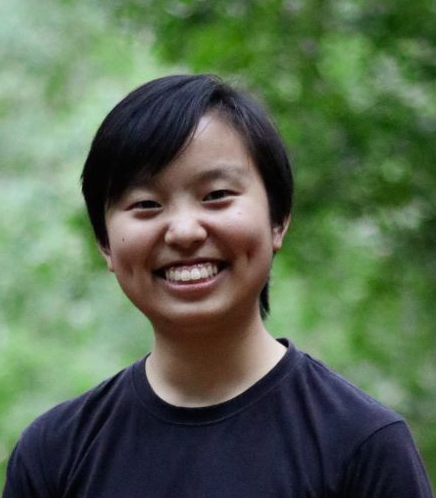
\includegraphics[scale=0.20]{dp_cropped}
\end{wrapfigure}
\fi

%----------HEADING----------

{\basictitle \Huge Arthur Goldblatt}
\\

% ----- TOGGLE FOR PHOTO ----
% \vspace{10pt}

\href{mailto:arthurgoldblatt@berkeley.edu}{
    \faEnvelope
    \thinspace \thinspace
    \myuline{arthurgoldblatt@berkeley.edu}} $|$
\href{https://www.linkedin.com/in/arthur-goldblatt-39719285/}{
    \faLinkedin
    \thinspace \thinspace        
    \myuline{arthur-goldblatt}} $|$
\href{https://github.com/arthurgoldblatt}{
    \faGithub
    \thinspace \thinspace
    \myuline{arthurgoldblatt}} $|$
\faPhone
\thinspace \thinspace
(510) 295-3358

%-----------EDUCATION-----------
\section{Education}
  \resumeSubHeadingListStart
    \resumeSubheading
      {University of Berkeley, California}{Berkeley}
      {B. Eng. Electrical Engineering and Computer Science}{Aug. 2018 -- May 2022}
      \resumeItemListStart
      
        \resumeItem{3.79 GPA}

      \resumeItemListEnd
      
  \resumeSubHeadingListEnd
  

%-----------PROJECTS-----------
\section{Coding Projects}
    \resumeSubHeadingListStart
    
    \iffalse
    %\iftrue
      \resumeProjectHeading
          {\href{https://docs.google.com/document/d/1KDkTLrHkdisztk3NpyClVIrR6Kd5y5qNf7zhpmSb16U/edit?usp=sharing}{\myuline{\textbf{Voice Controlled Car}}} $|$ \textit{Energia, TI Launchpad Circuitry}}{June-August 2020}
          \resumeItemListStart
            \resumeItem{Build robotic voice-controlled car, moves in different directions and distances depended on the worded command}
            \resumeItem{Utilize learning from control by establishing feedback and control using eigenvalue placement}
            \resumeItem{Build mic-board that records voice inputs using a DAC and ADC we also build}
            \resumeItem{Train car to classify commands and react according with unsupervised learning (Singular Value Decomposition & Principal Component Analysis)}
          \resumeItemListEnd
          \fi
          
      \resumeProjectHeading
          {\href{}{\myuline{\textbf{NumC}}} $|$ \textit{C, Python}}{May 2020}
          \resumeItemListStart
            \resumeItem{Emulate Numpy Functionality by writing methods in C}
            \resumeItem{Translate methods in C using Python’s C API reference}
            \resumeItem{Speed up code by using techniques such as SIMD and Caching}
            \resumeItem{Results in code that manipulates matrices up to 100x faster than Python without optimizations}
          \resumeItemListEnd
          
      \resumeProjectHeading
          {\href{}{\myuline{\textbf{Honest}}} $|$ \textit{Swift, Google Firebase, PHP, MySql}}{October 2019}
          \resumeItemListStart
            \resumeItem{Developed an IOS app in XCode using Swift and Google Firebase that scans QR codes for product authentication}
            \resumeItem{Generate unique QR codes on the merchant’s end and compile them into a sharable and downloadable pdf file}
            \resumeItem{Connect front end to back end with Google Firebase after running to some issues with using PHP and MySql}
            \resumeItem{Utilize the user’s camera to check if the QR code is in the database and therefore authentic}
          \resumeItemListEnd
          
      \resumeProjectHeading
          {\href{}{\myuline{\textbf{Pacman AI}}} $|$ \textit{Python}}{September 2019}
          \resumeItemListStart
            \resumeItem{Create a Python program that allows Pacman to solve complex mazes.}
            \resumeItem{Implement a variety of search algorithms (A*, UCS) along with determining consistent heuristics.}
            \resumeItem{Utilize stacks and priority queues to keep track of fringe for search problems.}
            \resumeItem{Optimize heuristic for finding nearest food by accounting for walls; performed 25\% better than expected.}
          \resumeItemListEnd
          
        \resumeProjectHeading
          {\href{}{\myuline{\textbf{Gitlet: Version Control System}}} $|$ \textit{Java}}{August 2019}
          \resumeItemListStart
            \resumeItem{Utilize Java to design and create a version control system similar to Git.}
            \resumeItem{Read in arguments from command line, allowing for the storage and access of the user’s files.}
            \resumeItem{Ensure persistence by serializing and writing files to the disk using Java’s Serializable Interface and java.io}
            \resumeItem{Organize the user’s files in directories by tagging them with their respective SHA-1 ID’s.}
            \resumeItem{Deal with merge conflicts by comparing SHA-1 IDs of committed files and editing file contents to flag conflict.}
          \resumeItemListEnd 
      
    \resumeSubHeadingListEnd




%\iffalse
\iftrue
%-----------EXPERIENCE-----------
\section{Experience}
  \resumeSubHeadingListStart
  
    \resumeSubheading
      {Academic Tutor}{Oct 2019 -- Present}
      {UC Berkeley}{remote, part time}
      \resumeItemListStart
        \resumeItem{Tutor students 1 on 1 for subjects such as Data Structures, Data Science, Linear Algebra, etc.}
        \resumeItem{Took CS 370 to learn about CS pedagogy}
        \resumeItem{Adapt to remote learning by using Zoom and screen sharing to help my students}
      \resumeItemListEnd
      
    \iffalse
    %\iftrue
    \resumeSubheading
      {Golf Attendant}{Jan 2021 -- Present}
      {Tilden Park Golf Course}{Berkeley, CA, part-time}
      \resumeItemListStart
        \resumeItem{Recruit and sign people up to the course's Players Club}
        \resumeItem{Manage the flow of golf carts}
        \resumeItem{Ensure we are not falling behind on the tee time schedule by making sure people tee off promptly without issue}
      \resumeItemListEnd
     \fi
      
\fi
      
      \iffalse
      % \iftrue
% -----------Multiple Positions Heading-----------
    \resumeSubSubheading
     {Software Engineer I}{Oct 2014 - Sep 2016}
    \resumeItemListStart
        \resumeItem{Apache Beam}
          {Apache Beam is a unified model for defining both batch and streaming data-parallel processing pipelines}
     \resumeItemListEnd
    \resumeSubHeadingListEnd
%-------------------------------------------

    \resumeSubheading
      {ESG Data Analyst}{May -- Aug 2018}
      {Schneider Electric}{Singapore}
      \resumeItemListStart
        \resumeItem{Optimised usage of in-house energy monitoring software and reaped energy savings of \$1,545 per month}
        \resumeItem{Created 12 other mini-deliverables; 10 were self-initiated. These include databases, guides, and reports, along with internal learning materials for EcoStruxure, Schneider Electric’s main product offer}
        \resumeItem{Founded the Singapore branch’s Green Committee}
        \resumeItem{Organised Global Environment Day activities for the staff}
      \resumeItemListEnd
      
      \iffalse
      % \iftrue
    \resumeSubheading
      {Consultant}{Feb 2017}
      {National Environment Agency}{Singapore}
      \resumeItemListStart
        \resumeItem{Reviewed 4 candidate topics for R\&D funding: found current research grants and current environment technology}
      \resumeItemListEnd
      
    \resumeSubheading
      {Innovation Consultant}{Dec 2016}
      {Land Transport Authority}{Singapore}
      \resumeItemListStart
        \resumeItem{Proposed folding seat solution increases train capacity by 13\%}
        \resumeItem{Achieved best presentation award (out of 9 pairs of people)}
      \resumeItemListEnd
\fi
\fi

  \resumeSubHeadingListEnd

\iffalse
%-----------RESEARCH-----------
\section{Research (papers linked)}
  \resumeSubHeadingListStart
  
    \resumeSubheading
      {\href{https://drive.google.com/open?id=1mmfRboc6VkFRZTedy0Wzz4gklM4_84w3}{\myuline{Rechargeable aqueous zinc batteries}}}{Aug 2018 -- Jun 2019}
      {with Prof Srinivasian Madhavi}{NTU, Singapore}
      \resumeItemListStart
        \resumeItem{Synthesised electrolytes, ran CVs \& three-electrode tests}
        \resumeItem{Published results in URECA (undergrad research) proceedings}
      \resumeItemListEnd
      
    \resumeSubheading
      {\href{https://drive.google.com/open?id=1U78X1NCEEXN3O1o8Wnd_czyM6F7XEFJh}{\myuline{Lithium ion battery anodes}}}{Dec 2017 -- May 2018}
      {with Prof Srinivasian Madhavi}{NTU, Singapore}
      \resumeItemListStart
        \resumeItem{Synthesised battery slurries}
        \resumeItem{Learned various techniques: XRD analysis, cyclic voltammetry, thermogravimetric analysis, hydrothermal synthesis, data analysis}
        \resumeItem{Published paper in ChemElectroChem (third author)}
        \begin{itemize}
            \item DOI: 10.1002/celc.201801244
        \end{itemize}
      \resumeItemListEnd
      
    \resumeSubheading
      {Dye-sensitised Solar Cells}{Apr -- Jul 2017}
      {with Associate Prof Soo Han Sen}{NTU, Singapore}
      \resumeItemListStart
        \resumeItem{Tested 4 experiment variables and conditions}
        \resumeItem{Increased scale of synthesis by 20\%}
      \resumeItemListEnd

  \resumeSubHeadingListEnd
  \fi

\iffalse
%-----------CCAs-----------
\section{Extracurriculars}
    \resumeSubHeadingListStart
    
      \resumeSubheading
      {Founder}{Jan 2018 -- present}
      {Breathe Easy NTU/Hazy Waste}{}
      \resumeItemListStart
        \resumeItem{Won \$5,000 grant to promote sustainable palm oil in Singapore}
        \resumeItem{Lead a team of 18 to \href{https://drive.google.com/file/d/1SHm7c42NkIvISBImdOo7QajR64gDjuw9/view}{\myuline{survey 237 students}} and \href{https://drive.google.com/file/d/1Y2rG_mDPt50KHoXztLaMhA1Tjk7pM_7E/view?usp=sharing}{\myuline{44 canteen vendors}} for their view on palm oil, producing 2 reports on the results}
        \resumeItem{Converted one canteen to sustainable palm oil; NUS followed suit}
      \resumeItemListEnd
    
      \resumeSubheading
          {Operations}{Jul 2018 -- Present}
          {Effective Altruism Singapore}{}
          \resumeItemListStart
            \resumeItem{Set up scalable Eventbrite ticketing platform with Zapier integration}
            \resumeItem{Facilitate inaugural Arete Fellowship in Singapore for Asia}
          \resumeItemListEnd
          
      \resumeSubheading
      {External Liaison Director}{Aug 2018 -- May 2019}
      {Earthlink NTU}{}
      \resumeItemListStart
        \resumeItem{Lead a team of 3 to organise 3 events and run 3 booths, with total turnout of 450 across the 6}
      \resumeItemListEnd
      
      \resumeSubheading
      {Assistant Head}{Jul 2018 -- Jul 2019}
      {ASEAN Youth Organization}{}
      \resumeItemListStart
        \resumeItem{Organised the ASEAN Youth Conference for roughly 100 ASEAN participants in an international team of 17}
      \resumeItemListEnd
          
    \resumeSubHeadingListEnd
\fi

\iffalse
%-----------PROGRAMMING SKILLS-----------
\section{Skills}
 \begin{itemize}[leftmargin=0.15in, label={}]
    \small{\item{
     \textbf{Languages}{: Python, C/C++, SQL, JavaScript, HTML/CSS, R} \\
     %\textbf{Developer Tools}{: Jupyter Notebooks, Git, Google Cloud Platform, VS Code, Amazon AWS} \\
     }
     }
 \end{itemize}
 \fi


%
%\iffalse
\iftrue
%-----------PROGRAMMING SKILLS-----------
\section{Technical Skills}
 \begin{itemize}[leftmargin=0.15in, label={}]
    \small{\item{
     \textbf{Languages}{: Python, Java, Go, C, SQL, Lisp, JavaScript, HTML/CSS} \\
     %\textbf{Frameworks}{: WordPress} \\
     \textbf{Developer Tools}{: Jupyter Notebooks, Git, Google Cloud Platform, X Code, Amazon AWS} \\
     \textbf{Libraries}{: pandas, plotly}
    }}
 \end{itemize}
\fi

%-------------------------------------------

%-----------INTERESTS-----------
\section{Interests}
\begin{itemize}[leftmargin=0.15in, label={}]
    \small{\item{
    Books (most recent: \textit{Just Mercy}) | Golf | Road Biking | Skiing | Tennis | Basketball | Stormy Weather | Tea 
    }}
 \end{itemize}
%-------------------------------------------
\end{document}
